\section{A compact family with independent parameters}\label{sec:geometry}

We first construct the compact family and fix the gauges used in the
analysis. The construction is classical pointed plumbing
\cite[\S8.3]{hubbard-koch}, with a particular choice of component metrics
and flat connections. The auxiliary markings will be forgotten without
contracting any component.

\subsection{The curve and its metrics}
Let $E$ be the smooth projective completion of
\[
 y^2=(x-1)(x-2)(x-3),
\]
and let $p,q$ be the two points over $x=0$. Take copies $E_+,E_-$ of
$E$ and copies $R_p,R_q$ of $\PP^1$. Join the two points named $p$ to
$0,\infty$ on $R_p$, and join the two points named $q$ to $0,\infty$
on $R_q$. The resulting nodal curve $C_0$ has dual graph $K_{2,2}$.
Its arithmetic genus is $1+1+1=3$. The points $1\in R_p,R_q$ make it a
stable two-pointed curve.

Choose disjoint coordinate disks at all eight branch points, using flat
coordinates on the elliptic curves and unitary M\"obius coordinates on
the rational curves. With the components and these coordinates fixed,
pointed plumbing gives a proper flat family
\begin{equation}\label{eq:plumbing}
 \pi:\cC\longrightarrow B=\Delta_\delta^4,
 \qquad u_ev_e=\tau_e\quad(e\in E(K_{2,2})).
\end{equation}
Here $E(K_{2,2})$ denotes the edge set, not the elliptic curve. All four
$\tau_e$ are independent. For clarity, choose fixed radii $0<a<b_0$
in the coordinate disks and $\delta<a^2$. The product component exteriors
are glued to the patches $|u_e|,|v_e|<b_0$ by
\[
 (u_e,\tau)\longmapsto
 (u_e,\tau_e/u_e,\tau_{f\ne e}),
\]
and the analogous map on the other branch. The two incidence overlaps of
one node are disjoint, since both $|u_e|>a$ and $|v_e|>a$ would imply
$|\tau_e|>a^2$. Different node patches are disjoint. There are no triple
incidence overlaps. Locally the total space has coordinates
$(u_e,v_e,\tau_{f\ne e})$ and is smooth. Every fibre with all
$\tau_e\ne0$ is a connected smooth compact curve of genus three.
Forgetting the two sections leaves the same proper family. In particular,
the rational bridges in $C_0$ remain present. Independence of these family
parameters makes no assertion about injectivity into unmarked moduli.

\begin{figure}[htbp]
\centering
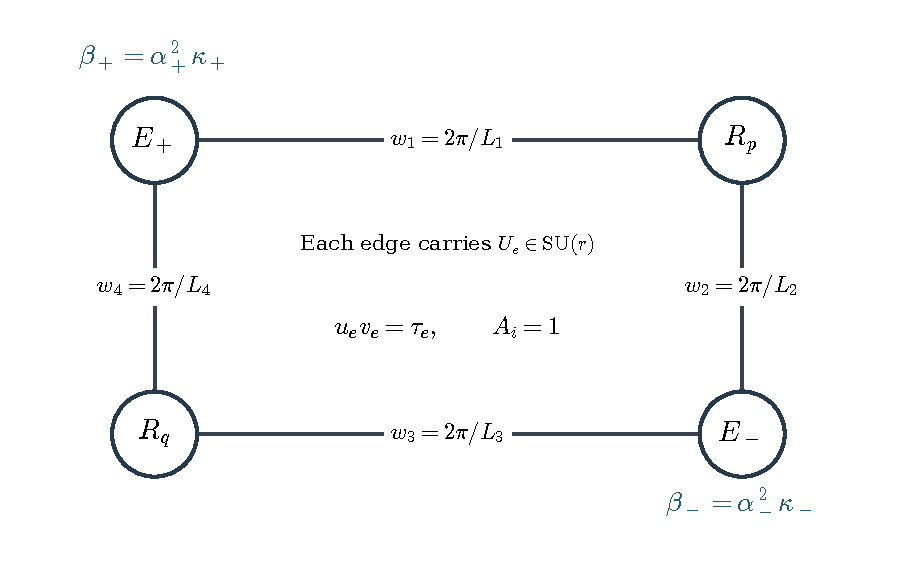
\includegraphics[width=\textwidth]{figures/output/fig02_family.pdf}
\caption{The four normalization components and their independent
parameters. The edge coefficients are $w_e=2\pi/L_e$ and the two
component coefficients are $\beta_i=\alpha_i^2\kappa_i$. The
rational bridges are retained in the compact family.}
\label{fig:family}
\end{figure}

Give $E_+,E_-$ their flat metrics of area one and $R_p,R_q$ their
Fubini--Study metrics of area one. Write $\omega_i^{\mathrm{area}}$ for
these K\"ahler forms and $A_i=1$ for their areas.

\begin{lemma}\label{lem:total-metric}
After shrinking $B$, the total space $\cC$ has a smooth K\"ahler form
whose restriction to each central normalization component is
$\omega_i^{\mathrm{area}}$. Each smooth fibre has area four. On a
sufficiently small node patch its fibre metric is the restriction of
$\omega_i^{\mathrm{area}}(u_e)+\omega_j^{\mathrm{area}}(v_e)$.
\end{lemma}

\begin{proof}
Choose on each component a degree-one holomorphic line bundle $L_i$ with
a Hermitian metric of Chern form $\omega_i^{\mathrm{area}}$. On an
elliptic component, start with any metric on a degree-one line bundle and
solve the scalar Poisson equation for the difference of the two curvature
forms. That difference has integral zero. Fourier series on the flat
torus give a smooth solution. On $\PP^1$, take $\mathcal O(1)$.
We use the convention in which a degree-one Chern form integrates to one.

In a holomorphic frame near a branch point write the squared norm as
$e^{-\psi_i(u)}$, with $\psi_i(0)=0$. On an elliptic branch a
holomorphic frame change removes the harmonic part of the potential,
leaving a positive multiple of $|u|^2$. On a rational branch the chosen
coordinate gives a positive multiple of $\log(1+|u|^2)$. In particular,
the first derivative of every $\psi_i$ vanishes at zero.

Glue the product line bundles on the component exteriors to a trivial
line on each node patch by these frames. The absence of triple incidence
overlaps verifies the cocycle condition. On a smaller node patch set the
squared norm of its frame equal to
\[
 \exp\{-\psi_i(u_e)-\psi_j(v_e)\}.
\]
On the $u_e$ overlap its ratio to the component metric is
$\exp\{-\psi_j(\tau_e/u_e)\}$. Interpolate the logarithm of this
ratio on a fixed incidence collar, leaving the product metric unchanged
outside it. The resulting smooth metric on the line bundle has Chern
form $\Omega$. Along a central branch the correction and all its
tangential derivatives vanish, so its restriction is exactly the
prescribed component form. On the smaller node patches its curvature is
the sum of the two branch forms.

Let $\omega_B$ be the Euclidean form on $B$. Near a node,
$\Omega+C\pi^*\omega_B$ is positive for every $C>0$: the branch
forms control the $u_e,v_e$ directions and the base form controls the
remaining three coordinates. On the compact remainder of the central
fibre, $\pi$ is a submersion and $\Omega$ is strictly positive on the
vertical tangent. In finitely many submersion charts, a Schur-complement
estimate makes $\Omega+C\pi^*\omega_B$ positive for one sufficiently
large $C$. Properness and a smaller $B$ make these neighborhoods cover
every fibre. The form is closed and of type $(1,1)$, hence K\"ahler.
Its fibre restrictions do not depend on the added base form. The degree
of the line bundle on every smooth fibre is $\sum_i\deg L_i=4$.
\end{proof}

Write $dA_\tau$ for this fibre area form and define
\begin{equation}\label{eq:parameters}
 L_e=\log(1/|\tau_e|),\quad L_* =\min_e L_e,\quad
 \epsilon_e=L_e^{-1},\quad \epsilon_* =L_*^{-1},\quad
 b=\max_e|\tau_e|=e^{-L_*}.
\end{equation}
All limits below have $L_*\to\infty$.

\begin{lemma}\label{lem:geometric-estimates}
Choose a radius $\rho$ with $b<\rho^2$. The middle annulus of node
$e$, given by $|\tau_e|/\rho<|u_e|<\rho$, has area at most
$C\rho^2$, independently of its modulus. Its scalar Dirichlet capacity
is
\begin{equation}\label{eq:capacity}
 \frac{2\pi}{L_e+2\log\rho}.
\end{equation}
The punctured component $|u_e|\ge\rho$ has a natural holomorphic
identification with its image in $C_\tau$. For every fixed derivative
order $m$, its fibre metric differs from the component metric by at most
$C_m b^2\rho^{-N_m}$ in that order, for some finite $N_m$.
\end{lemma}

\begin{proof}
The two branch terms in Lemma~\ref{lem:total-metric} each integrate
over a disk of radius $\rho$, proving the area bound. In complex
dimension one the Dirichlet integral is conformally invariant. The
radial harmonic function between the two boundary circles is affine in
$\log|u_e|$, and direct integration of its squared derivative gives
\eqref{eq:capacity}. In the branch identification, $v_e=\tau_e/u_e$.
Differentiating this identity in the fixed branch potentials gives the
stated polynomial losses in $\rho^{-1}$ and the factor $|\tau_e|^2$.
On the fixed interpolation collars the denominators are bounded, and
outside them the metric agrees with the product metric. No inverse power
of an individual $\tau_e$ occurs. In particular $\rho=L_*^{-1}$
makes every required error tend to zero.
\end{proof}

\subsection{The flat bundle}
Fix $r\ge2$, trace-free Hermitian matrices $T_+,T_-$, and nonzero real
harmonic one-forms $\vartheta_+,\vartheta_-$ on the two flat elliptic
curves. For two small real numbers $\alpha_+,\alpha_-$ set
\begin{equation}\label{eq:component-connection}
 D_i=d-i\alpha_iT_i\vartheta_i\quad(i=+,-),
 \qquad D_i=d\quad(i=p,q),
 \qquad \kappa_i=\int_{E_i}|\vartheta_i|^2\,dA_i.
\end{equation}
The elliptic connections are expressed in global smooth unitary frames.
Their curvature and determinant connection vanish. Near an elliptic
branch point the primitive of $\vartheta_i$ vanishing at the point is
\begin{equation}\label{eq:primitive}
 F_{ie}(u)=c_{ie}^{\mathrm{harm}}u+
           \overline{c_{ie}^{\mathrm{harm}}u}.
\end{equation}
This identity is exact: the coordinates are flat and the harmonic
one-form is constant. The change of frame
$G_{ie}=\exp(i\alpha_iT_iF_{ie})$ is unitary and gives a parallel
frame. On rational branches put $G_{ie}=I$.

Fix unitary matrices $U_{ij}\in\SU(r)$ on oriented edges, with
$U_{ji}=U_{ij}^{-1}$. We use the convention that they carry the
$j$-end data to the $i$-end frame. Glue a trivial flat bundle on each
node patch to the component local systems using constant identifications
in these parallel frames, with relative matrix $U_{ij}$.

\begin{proposition}\label{prop:bundle-family}
For every fixed $\alpha=(\alpha_+,\alpha_-)$ these identifications
define a flat unitary connection $D$ and parallel determinant on a
holomorphic vector bundle over the whole smooth total space $\cC$.
They depend smoothly on $\alpha$. The four complex parameters $\tau_e$
and the two real parameters $\alpha_i$ vary independently. The parallel
Hermitian metric $h_0$ restricts to an HYM metric of slope zero on every
smooth fibre.
\end{proposition}

\begin{proof}
Pull each component connection back to its product exterior, taking the
full exterior derivative there. It is flat. On every incidence overlap,
the designated frames are parallel, and the constant node
identifications are isomorphisms of flat connections. There are no
triple incidence overlaps. The connections and metrics therefore glue.
Flatness implies $(D^{0,1})^2=0$, so local parallel frames are
holomorphic and define the asserted locally free bundle on $\cC$.
All transition maps have determinant one. This construction uses no
relation between $\alpha$ and $\tau$ and depends smoothly on the real
parameters. We assert holomorphic dependence on $\tau$ for each fixed
$\alpha$, not a flat connection in the additional real parameter
directions. The fibrewise Chern curvature of $h_0$ vanishes.
\end{proof}

\subsection{Stability and parallel endomorphisms}
Shrinking the allowed $\alpha$ interval once, the parallel trace-free
Hermitian endomorphisms of $D$ are exactly the tuples satisfying
\begin{equation}\label{eq:common-kernel}
 X_i=\Ad(U_{ij})X_j\quad(e=ij),\qquad
 \alpha_i[T_i,X_i]=0\quad(i=+,-).
\end{equation}
Indeed, choose a nonzero period of $\vartheta_i$. For sufficiently small
nonzero $\alpha_i$, distinct eigenvalues of $T_i$ remain distinct
after exponentiation by that period. Its holonomy commutant is thus the
commutant of $T_i$. A commuting endomorphism is constant in the harmonic
gauge and in each node-normalized parallel frame. Node compatibility is
precisely the first equation of \eqref{eq:common-kernel}. When
$\alpha_i=0$ the second equation is vacuous.

The unitary-flat correspondence \cite{narasimhan-seshadri} makes every
smooth-fibre bundle polystable of degree zero. It is stable exactly when
\eqref{eq:common-kernel} has no nonzero solution. Equivalently, the
degree formula for a holomorphic subbundle expresses its degree as the
negative squared norm of its second fundamental form. Equality forces a
parallel orthogonal splitting. Conversely a nonzero trace-free Hermitian
commutant supplies such a splitting by its eigenspaces.

For an explicit transition in rank two, let
\begin{equation}\label{eq:pauli-data}
 T_+=\sigma_z=\begin{pmatrix}1&0\\0&-1\end{pmatrix},\qquad
 \alpha_-=0,\qquad
 U=\frac{I+i\sigma_x}{\sqrt2},\qquad
 \sigma_x=\begin{pmatrix}0&1\\1&0\end{pmatrix}.
\end{equation}
Take the identity on a spanning tree and $U$ on the remaining edge.
Tree compatibility makes all $X_i$ equal. For $\alpha_+\ne0$, the
component commutant is the $\sigma_z$ axis, whereas the cycle edge
fixes the $\sigma_x$ axis. Their intersection is zero. At
$\alpha_+=0$ the latter axis survives. Thus the same compact family is
stable for sufficiently small $\alpha_+\ne0$ and strictly polystable
at $\alpha_+=0$.

The component and cycle operations in this example do not commute.
To interpret cycle holonomy, fix basepoints and paths to the nodes.
The resulting based holonomy includes component path factors
$\exp(i\alpha_iT_i\int\vartheta_i)$ as well as the $U_{ij}$.
A product of node matrices alone is not generally the based holonomy.
The family changes holomorphic stability by changing the bundle, not
by changing the polarization of a curve. Its underlying smooth
$\SU(r)$ bundle is topologically trivial; no unstable locus is
claimed.
